The SIERHD model from the August monthly demo uses the model summarized by the Petrinet diagram in Figure \ref{fig:seirhd}.

\begin{figure}
    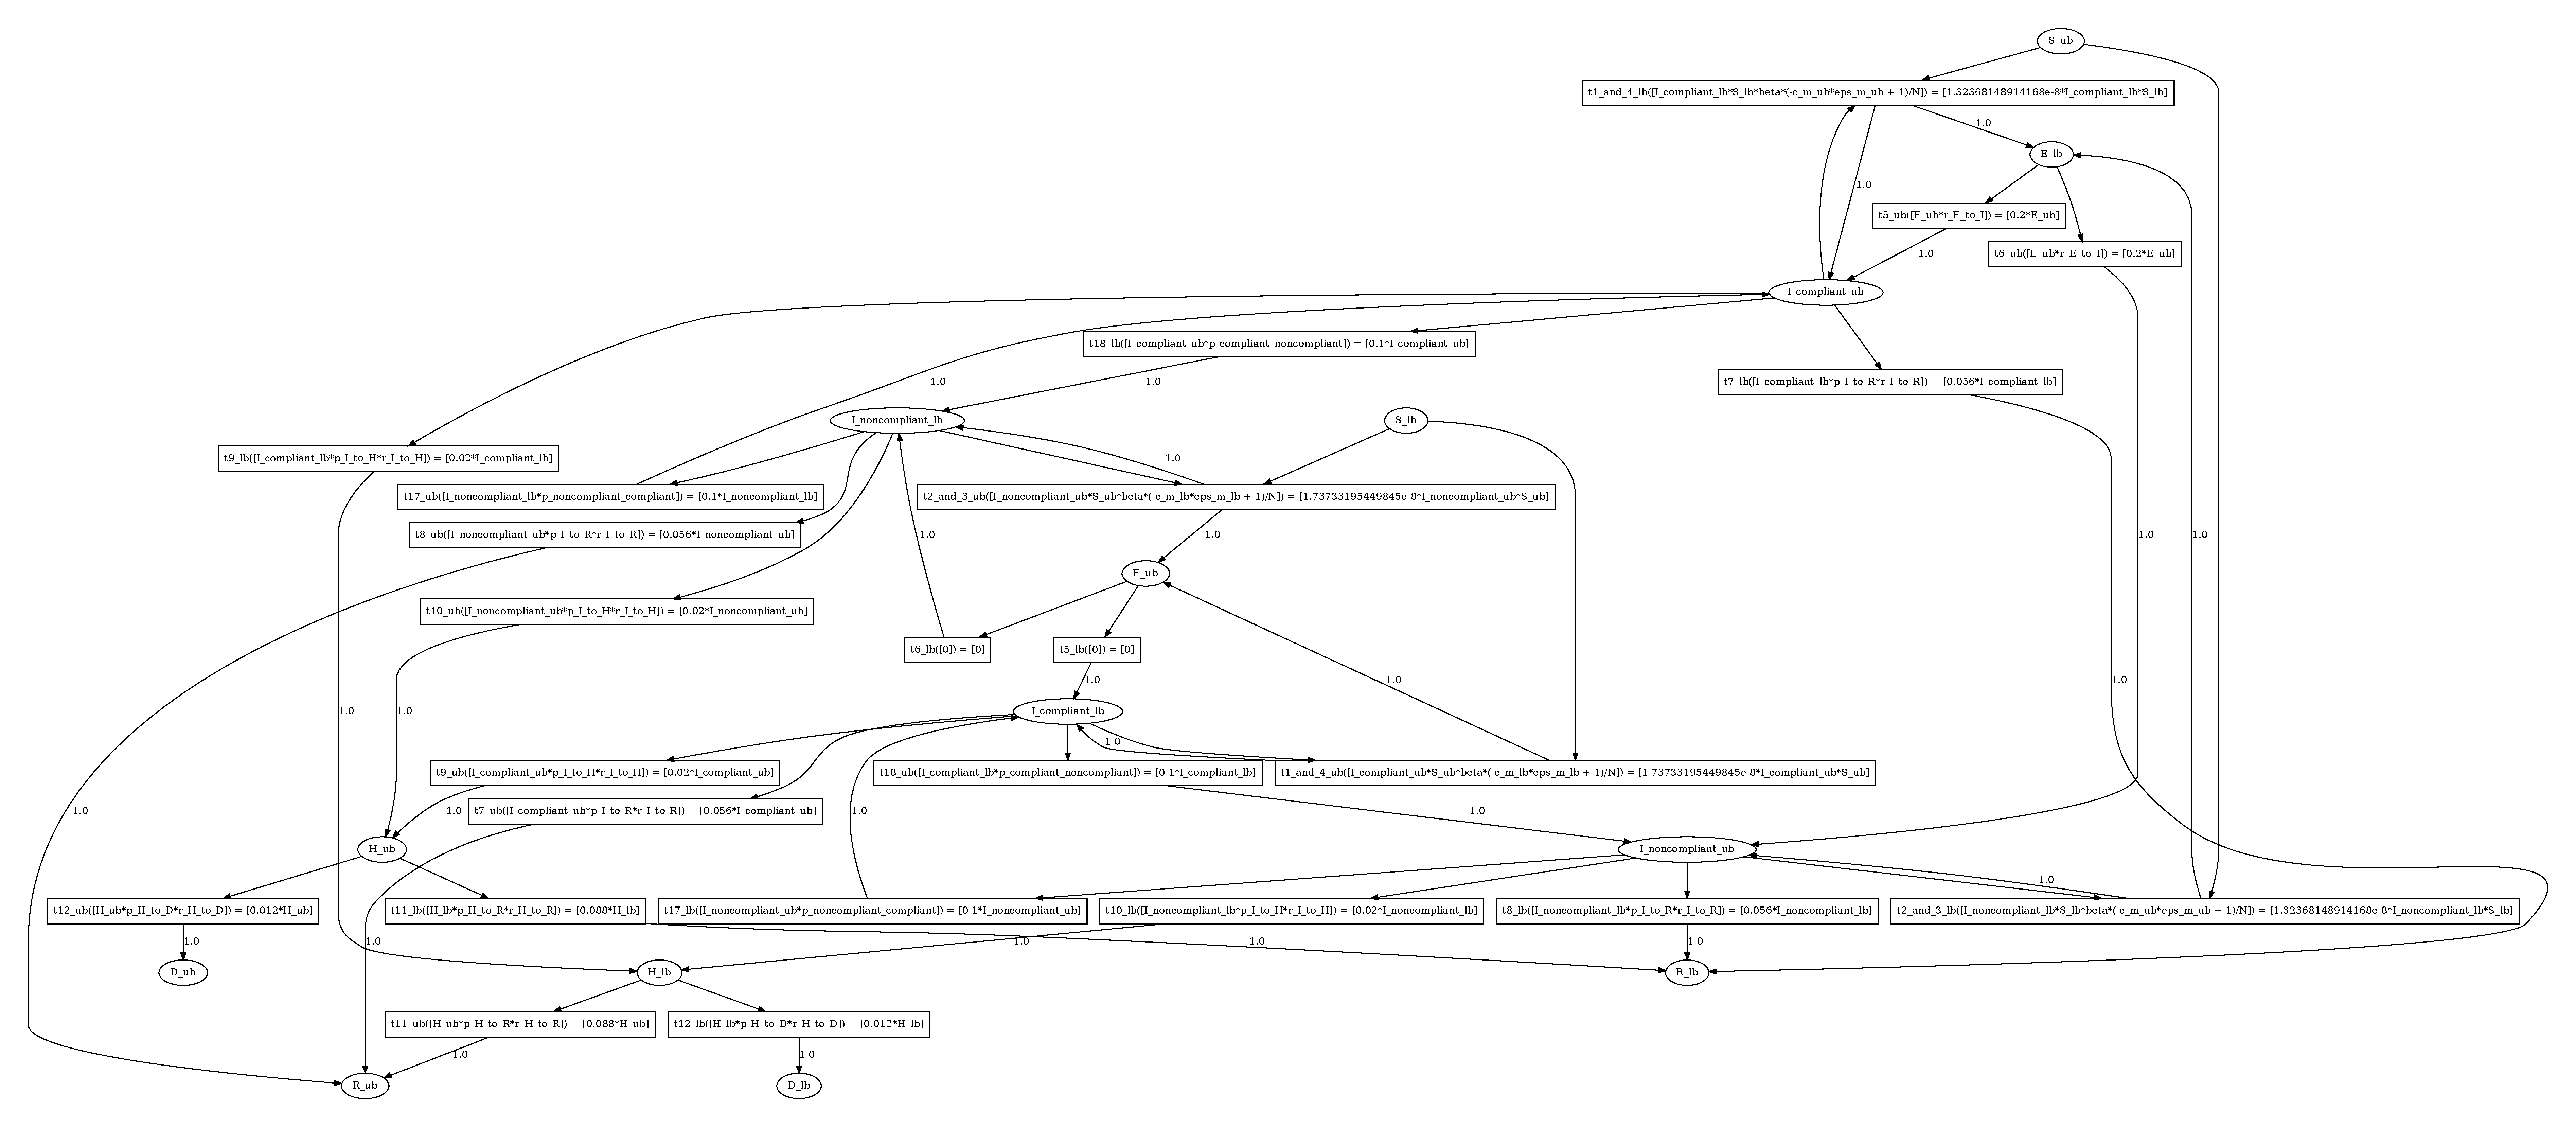
\includegraphics[width=\linewidth]{fig/seirhd-aug}
    \caption{\label{fig:seirhd} SEIRHD Model Petrinet}
\end{figure}

The following transitions connect the variables $S_c$, $S_{nc}$, $E_c$, $E_{nc}$, $I_c$, and $I_{nc}$, $R$, $H$, $D$:

\begin{eqnarray*}
    t_1: (I_c, S_c) &\xrightarrow[]{r_1}& (I_c, E_c) \\
    t_2: (I_{nc}, S_c) &\xrightarrow[]{r_2}& (I_{nc}, E_c)\\
    t_3: (I_{nc}, S_{nc}) &\xrightarrow[]{r_3}& (I_{nc}, E_{nc})\\
    t_4: (I_c, S_{nc}) &\xrightarrow[]{r_4}& (I_c, E_{nc})\\
    t_5: (E_c) &\xrightarrow[]{r_5}& (I_c)\\
    t_6:(E_{nc}) &\xrightarrow[]{r_6}& (I_{nc})\\
    t_7:(I_c) &\xrightarrow[]{r_7}& (R)\\
    t_8: (I_{nc}) &\xrightarrow[]{r_8}& (R)\\
    t_9:(I_c) &\xrightarrow[]{r_9}& (H)\\
    t_{10}:(I_{nc}) &\xrightarrow[]{r_{10}}& (H)\\
    t_{11}:(H) &\xrightarrow[]{r_{11}}& (R)\\
    t_{12}:(H) &\xrightarrow[]{r_{12}}& (D)\\
    t_{13}:(S_{nc}) &\xrightarrow[]{r_{13}}& (S_c)\\
    t_{14}:(S_c) &\xrightarrow[]{r_{14}}& (S_{nc})\\
    t_{15}:(E_{nc}) &\xrightarrow[]{r_{15}}& (E_c)\\
    t_{16}:(E_c) &\xrightarrow[]{r_{16}}& (E_{nc})\\
    t_{17}:(I_{nc}) &\xrightarrow[]{r_{17}}& (I_c)\\
    t_{18}:(I_c) &\xrightarrow[]{r_{18}}& (I_{nc})
\end{eqnarray*}

Abstracting this base model involves merging variables, such as $S_c$ and $S_{nc}$ into a composite variable $S$ where $S = S_c + S_{nc}$.  In this approach, a composite variable can represent any number of stratified copies of a variable (e.g., $S$ stratified by ten age groups). We also abstract the base model transitions so that their source and target variables are composite variables.  For example, if we define composite variables $S$, $I$, and $E$ for the corresponding stratified variables in the base model, then transitions $t_1$ to $t_4$ become the composite transition $t_{1:4}$:

\begin{eqnarray*}
    t_{1:4}:(I, S) &\xrightarrow[]{r_{1:4}}& (I, E)
\end{eqnarray*}

\noindent where $r_{1:4}$ is the composite rate of flow and $r_{1:4} = \sum_{i=1}^4 r_i$.  The composite rate of flow $r_{1:4}$ between the base variables due to the base transitions becomes difficult to track because we no longer separately model each base variable.  For example $r_1 = \frac{I_c S_c \beta(-c_{m_0}*\epsilon_{m_0} + 1)}{N}$, depends upon $I_c$ and $S_c$, and they are no longer variables in the abstract model.  We express $r_{1:4}$ in terms of the abstract variables by bounding it.  Bounding the rate expressions implies that we must also bound each of the variables.  We denote the upper and lower bounds with the $ub$ and $lb$ superscripts. 

For example, we express the rate $r_{1:4}$ with a pair of rates $r^{lb}_{1:4}$ and $r^{ub}_{1:4}$.  If we assume that the composite rate preserves the total flow between base model variables, we define bounds on the rate as follows: 

\begin{eqnarray*}
    S(t+dt) &=& S_c(t+dt) + S_{nc}(t+dt)\\
    &=& S_c(t) - (r_1+ r_2)dt  + S_{nc}(t) - (r_3+ r_4)dt\\
    &=& S(t) - (r_1+ r_2 +r_3+ r_4)dt\\
    &=& S(t) - \biggl(\frac{I_c S_c \beta(1-c_{m_0}\epsilon_{m_0})}{N}+\frac{I_{nc} S_c \beta(1-c_{m_1}\epsilon_{m_1} )}{N}+\\
    &&\qquad\qquad\frac{I_{nc} S_{nc} \beta(1-c_{m_2}\epsilon_{m_2} )}{N}+\frac{I_c S_{nc} \beta(1-c_{m_3}\epsilon_{m_3} )}{N}\biggl)dt\\
    &\leq& S(t) - \biggl(\frac{I_c S_c \beta(1-c^{ub}_{m}\epsilon^{ub}_{m}  )}{N}+\frac{I_{nc} S_c \beta(1-c^{ub}_{m}\epsilon^{ub}_{m})}{N}+\\
    &&\qquad\qquad\frac{I_{nc} S_{nc} \beta(1-c^{ub}_{m}\epsilon^{ub}_{m})}{N}+\frac{I_c S_{nc} \beta(1-c^{ub}_{m}\epsilon^{ub}_{m} )}{N}\biggl)dt\\
    &=& S(t) - \frac{\beta(1-c^{ub}_{m}\epsilon^{ub}_{m} )}{N}(I_c S_c +I_{nc} S_c +I_{nc} S_{nc} +I_c S_{nc} )dt\\
    &=& S(t) - \frac{\beta(1-c^{ub}_{m}\epsilon^{ub}_{m} )}{N}((I_c+I_{nc}) (S_c + S_{nc}) )dt\\
    &=& S(t) - \frac{\beta(1-c^{ub}_{m}\epsilon^{ub}_{m} )}{N}(IS)dt\\
    &\leq& S^{ub}(t) - \frac{I^{lb}S^{lb}\beta(1-c^{ub}_{m}\epsilon^{ub}_{m} )}{N}dt\\
    &=& S^{ub}(t+dt)
    % &&
\end{eqnarray*}

\noindent where the upper bound $S^{ub}(t+dt)$ assumes that the negative rate terms have minimal magnitude (i.e., the upper bound decreases by the least amount). The terms are minimal when they are replaced by the appropriate bounds $I^{lb}$, $S^{lb}$, $c^{ub}_{m}$, $\epsilon^{ub}_{m}$.  The lower bound $S^{ub}(t+dt)$ uses a similar approach, instead selecting bounds with a maximum magnitude and decreasing the lower bound by greatest amount.  Positive rate terms are handled similarly so that they are maximal when used to compute upper bounds and minimal for lower bounds.

The abstract model that de-stratifies the base model defines 12 compartments (lower and upper bound for each variable after defining the composite variables), and 12 transitions (lower and upper bound for each composite transition).  While the resulting model has fewer transitions, it has more compartments.  However, we would have constructed the same size abstraction for a stratified model with an arbitrary number of levels.  For example, if the base model used ten levels instead of two, then it would have 33 compartments and significantly more transitions.  

We developed two abstract models from the base model.  The first, as described above, de-stratifies the $S$, $E$, and $I$ variables.  The second, de-stratifies only $S$ and $E$, allowing $I$ to remain stratified.  

\begin{figure}
    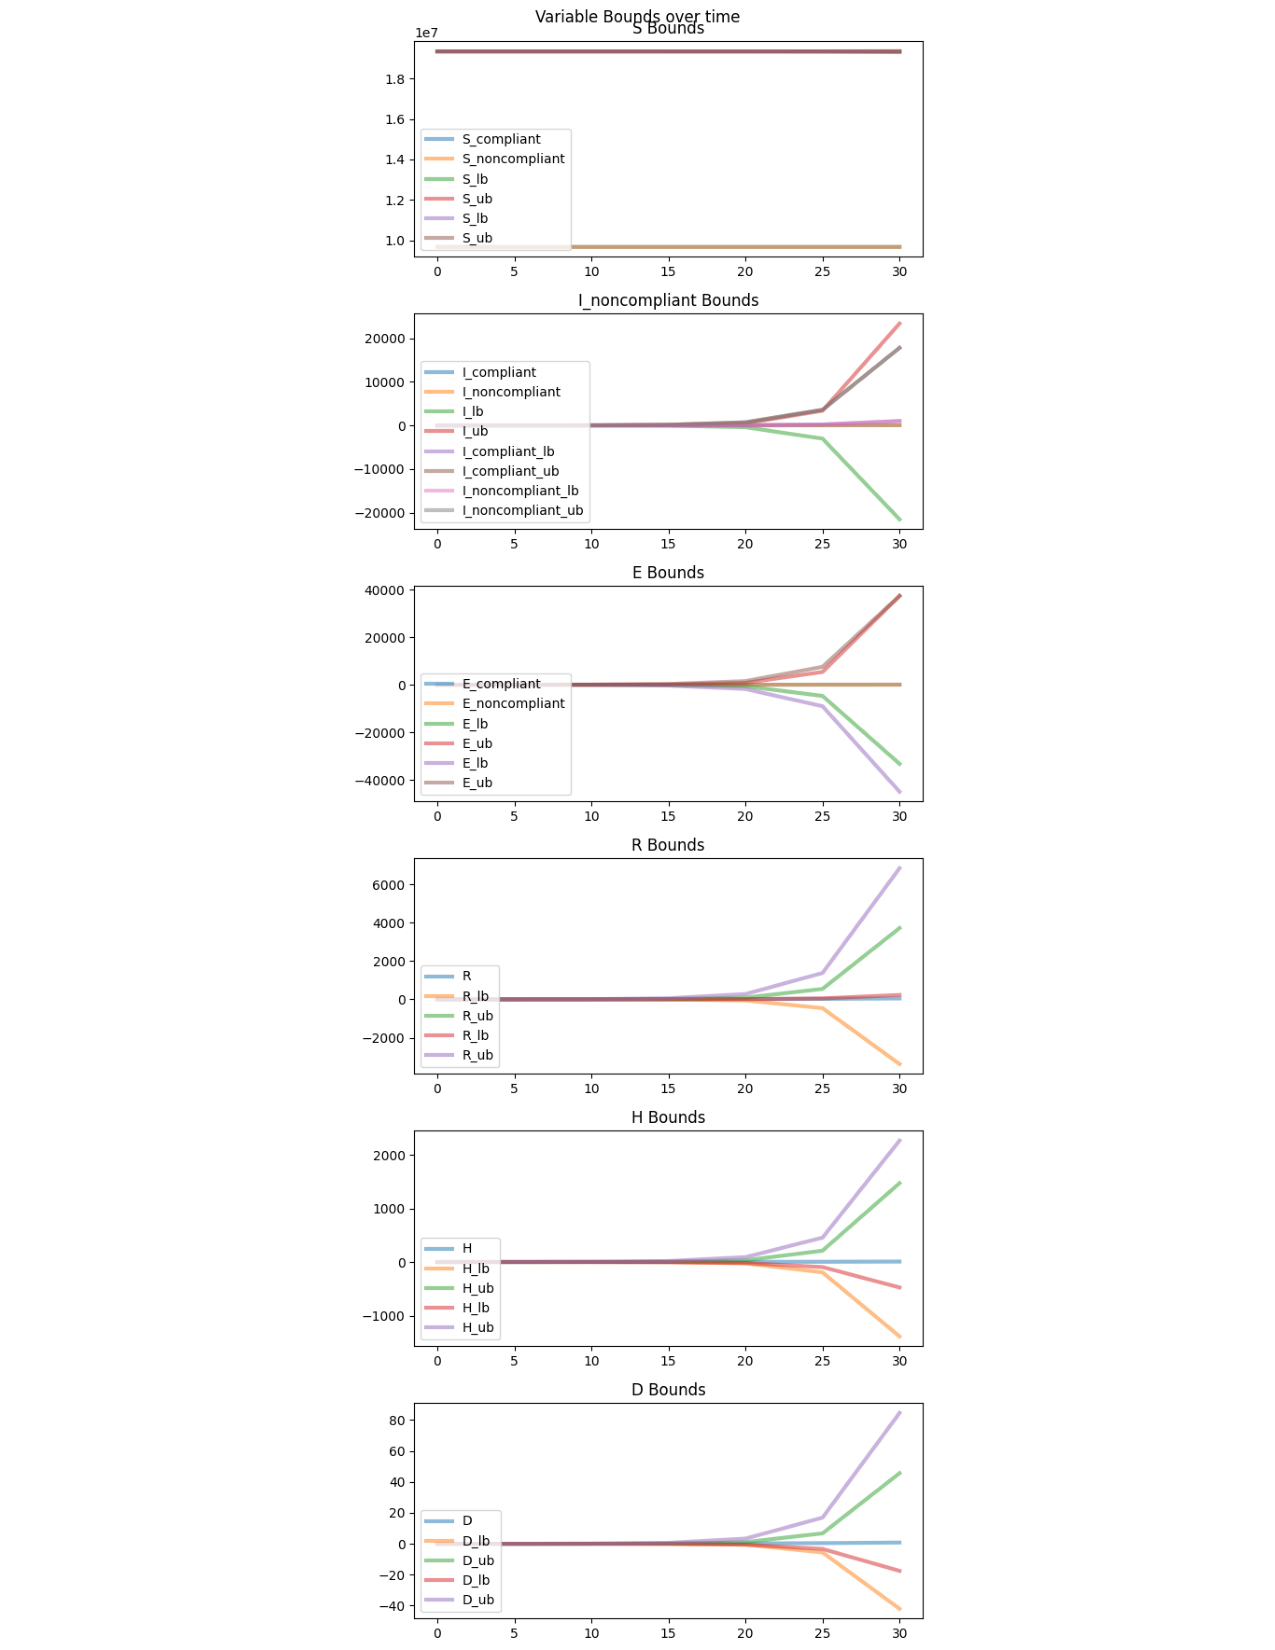
\includegraphics[width=\linewidth]{fig/seirhd_bounds.pdf}
    \caption{\label{fig:seirhd-bounds} SEIRHD Model Bounds}
\end{figure}

Figure \ref{fig:seirhd-bounds} illustrates the bounds computed by simulating the base and abstract models with FUNMAN.  Each subplot is one compartment variable, and each series is one of the bounds or base model value.  For example, the second plot illustrates $I$, which includes:
\begin{itemize}
    \item Base model: $I$\_compliant and $I$\_\text{noncompliant}, 
    \item De-stratified $S$, $E$, and $I$:  $I$\_\text{lb} and $I$\_\text{ub},
     \item De-stratified $S$, and $E$:  $I$\_compliant\_lb, $I$\_compliant\_ub,$I$\_noncompliant\_lb and $I$\_noncompliant\_ub,
\end{itemize}
The abstractions provide different bounds for each variable.  In general, as abstraction increases, the model will provide looser bounds, but with a smaller model.  Using abstraction refinement techniques, it is possible to start with an abstract model and only refine the relevant variables.  Selectively refining models will trade off multiple abstract model simulations against a single, potentially large model simulation.  In cases where the bounds are enough to answer a query (or check a constraint), the abstract model simulation can lead to significant scale up.  